\chapter{Funkcje patologiczne}
\label{ma1:ch:pathological-functions}

Przykłady w tym rozdziale oddzielają własności, które dla najprostszych funkcji występują razem: ciągłość, istnienie granic jednostronnych, monotoniczność i własność Darboux. W szczególności gęstość zbioru nieciągłości nie wyklucza ciągłości w innych punktach, a przyjmowanie wszystkich wartości pośrednich nie wymusza ciągłości bez dodatkowych założeń.

\section{Funkcje Dirichleta i Thomae'a}
\begin{przyklad}[Funkcja Dirichleta]
\label{ma1:ex:dirichlet}
Niech $D:\R\to\R$ będzie dana wzorem $D(x)=\chi_{\Q}(x)$. Funkcja $D$ nie ma granicy w żadnym punkcie i jest wszędzie nieciągła.
\end{przyklad}
\begin{proof}
Dla dowolnego $p\in\R$ z gęstości liczb wymiernych i niewymiernych wybieramy $r_n\in\Q\cap(p,p+1/n)$ oraz $s_n\in(\R\setminus\Q)\cap(p,p+1/n)$. Oba ciągi dążą do $p$, a żaden ich wyraz nie jest równy $p$. Mamy $D(r_n)=1$ i $D(s_n)=0$. Kryterium ciągowe granicy (twierdzenie \ref{ma1:thm:function-limit-sequential}) wyklucza istnienie granicy, a kryterium ciągowe ciągłości wyklucza ciągłość. Wybór punktów z lewej strony daje również nieistnienie obu granic jednostronnych.
\end{proof}

\begin{przyklad}[Funkcja Thomae'a]
\label{ma1:ex:thomae}
Definiujemy $T:\R\to[0,1]$ przez
\[
 T(x)=
 \begin{cases}
 1/q,& x=p/q,\ p\in\Z,\ q\in\N,\ q\ge1,\ \gcd(|p|,q)=1,\\
 0,&x\notin\Q.
 \end{cases}
\]
Ułamek nieskracalny o dodatnim mianowniku jest jednoznaczny; w szczególności $T(0)=1$. Dla każdego $a\in\R$ istnieje granica przekłuta $\lim_{x\to a}T(x)=0$. Zatem $T$ jest ciągła dokładnie w punktach niewymiernych.
\end{przyklad}
\begin{proof}
Ustalmy $a\in\R$ i $\varepsilon>0$. Wybierzmy całkowite $N\ge1$ z $1/N<\varepsilon$. Zbiór
$E_N=\{p/q\in[a-1,a+1]:p\in\Z,\ 1\le q\le N,\ \gcd(|p|,q)=1\}$
jest skończony: dla każdego z skończenie wielu mianowników $q$ licznik należy do ograniczonego przedziału $[q(a-1),q(a+1)]$. Przyjmijmy $\delta$ jako minimum liczby $1$ i wszystkich dodatnich odległości $|r-a|$ dla $r\in E_N\setminus\{a\}$. Jeśli ten ostatni zbiór jest pusty, przyjmujemy $\delta=1$. Mamy $\delta>0$.

Dla $0<|x-a|<\delta$ punkt $x$ należy do $[a-1,a+1]$, ale nie do $E_N$. Jeśli $x$ jest niewymierny, to $T(x)=0$; jeśli jest wymierny, jego nieskracalny mianownik jest większy od $N$, więc $0<T(x)<1/N<\varepsilon$. Dowodzi to granicy przekłutej. Ponieważ każdy punkt $\R$ jest punktem skupienia dziedziny, ciągłość jest równoważna $T(a)=0$, czyli $a\notin\Q$.
\end{proof}
\begin{center}
\begin{tikzpicture}[x=9cm,y=2.7cm,>=Stealth]
 \draw[->] (-.03,0)--(1.08,0) node[right] {$x$};
 \draw[->] (0,-.08)--(0,1.15) node[above] {$y$};
 \foreach \q in {1,...,11}{
  \foreach \p in {0,...,\q}{
   \pgfmathtruncatemacro{\g}{gcd(\p,\q)}
   \ifnum\g=1
    \fill[blue!65!black] ({\p/\q},{1/\q}) circle (.9pt);
   \fi
  }
 }
 \node[below] at (0,0) {$0$};
 \node[below] at (1,0) {$1$};
 \node[left] at (0,1) {$1$};
 \node[blue!65!black,above] at (.5,.5) {$1/2$};
\end{tikzpicture}

\small Rysunek: wartości funkcji Thomae'a dla nieskracalnych mianowników nie większych niż $11$; pominięto wartości o większych mianownikach i wartości zerowe w punktach niewymiernych.
\end{center}

\section{Oscylacje i własność Darboux}
\begin{przyklad}
\label{ma1:ex:oscillatory-darboux}
Niech $f(0)=0$ i $f(x)=\sin(1/x)$ dla $x\ne0$. Funkcja $f$ jest ciągła poza zerem, nie ma w zerze żadnej granicy jednostronnej i ma własność Darboux na $\R$.
\end{przyklad}
\begin{proof}
Ciągłość poza zerem wynika z ciągłości złożenia. Dla $n\ge1$ punkty $u_n=1/(\pi/2+2n\pi)$ i $v_n=1/(3\pi/2+2n\pi)$ dążą do zera z prawej, a $f(u_n)=1$ i $f(v_n)=-1$. Z nieparzystości $f$ analogiczne świadki po lewej to $-u_n,-v_n$. Granice jednostronne nie istnieją.

Niech $a<b$. Jeśli $0\notin[a,b]$, stosujemy twierdzenie o wartości pośredniej. Jeśli $0\in[a,b]$, przedział zawiera albo odcinek $[0,d]$ z $d>0$, albo $[-d,0]$ z $d>0$. W pierwszym przypadku dla dostatecznie dużego $n$ oba $u_n,v_n$ należą do $(0,d)$, a $f$ jest ciągła na przedziale o tych końcach. Przyjmuje tam wszystkie wartości z $[-1,1]$. W drugim przypadku stosujemy ten sam argument do $-u_n,-v_n$. Ponieważ $f$ nie przyjmuje wartości spoza $[-1,1]$, obraz $[a,b]$ zawierającego zero jest dokładnie $[-1,1]$. W każdym przypadku wszystkie wartości między $f(a)$ i $f(b)$ są osiągane na $[a,b]$.
\end{proof}

\begin{przyklad}
\label{ma1:ex:damped-oscillations}
Dla $\alpha>0$ funkcja $g_\alpha(x)=|x|^\alpha\sin(1/x)$ dla $x\ne0$ i $g_\alpha(0)=0$ jest ciągła na $\R$. Istotnie, $|g_\alpha(x)|\le |x|^\alpha$ i prawa strona dąży do zera. Nie jest jednak monotoniczna w żadnym otoczeniu zera.
\end{przyklad}
\begin{proof}
Wystarczy rozważyć dowolny przedział $(0,d)$, $d>0$. Dla dostatecznie dużego $n$ mamy $0<u_{n+1}<v_n<u_n<d$, gdzie $u_n,v_n$ pochodzą z poprzedniego przykładu. Wartości $g_\alpha(u_{n+1}),g_\alpha(u_n)$ są dodatnie, a $g_\alpha(v_n)$ ujemna. Trzy uporządkowane argumenty wykluczają zarówno niemalejący, jak i nierosnący charakter funkcji.
\end{proof}
\begin{center}
\begin{tikzpicture}[x=9cm,y=1.4cm,>=Stealth]
 \draw[->] (-.03,0)--(1.08,0) node[right] {$x$};
 \draw[->] (0,-1.2)--(0,1.25) node[above] {$y$};
 \draw[gray,dashed] (0,0)--(1,1) node[right] {$x$};
 \draw[gray,dashed] (0,0)--(1,-1) node[right] {$-x$};
 \draw[blue!65!black,thick,domain=.035:1,samples=350] plot (\x,{\x*sin(1/\x r)});
 \fill[blue!65!black] (0,0) circle (1.5pt);
\end{tikzpicture}

\small Rysunek: tłumione oscylacje $x\sin(1/x)$ dla $x>0$; dla czytelności nie rysowano oscylacji przy $0<x<0{,}035$.
\end{center}

\section{Zbiór Cantora}
\begin{definicja}
\label{ma1:def:cantor-set}
Niech $C_0=[0,1]$. Zbiór $C_{n+1}$ powstaje z $C_n$ przez usunięcie otwartej środkowej trzeciej części każdego przedziału składowego $C_n$. Zbiorem Cantora nazywamy $C=\bigcap_{n=0}^\infty C_n$.
\end{definicja}
Indukcyjnie $C_n$ jest sumą $2^n$ parami rozłącznych przedziałów domkniętych długości $3^{-n}$. Suma ich długości wynosi $(2/3)^n$. Nie jest to jeszcze definicja miary; wykorzystujemy wyłącznie długości skończenie wielu przedziałów.

\begin{twierdzenie}
\label{ma1:thm:cantor-properties}
Zbiór $C$ jest domknięty, ograniczony, nieprzeliczalny, nie ma punktów izolowanych i ma puste wnętrze w $\R$.
\end{twierdzenie}
\begin{proof}
Każdy $C_n$ jest domknięty jako skończona suma przedziałów domkniętych. Ich przecięcie jest domknięte: jeśli $x\notin C$, istnieje $n$ z $x\notin C_n$, a otwarte dopełnienie $C_n$ jest otoczeniem $x$ rozłącznym z $C$. Mamy $C\subseteq[0,1]$, a $0,1\in C$.

Końce każdego przedziału składowego $C_n$ pozostają we wszystkich kolejnych etapach, więc należą do $C$. Dla $x\in C$ wybieramy przedział składowy $C_n$ zawierający $x$. Co najmniej jeden z jego końców $y_n$ jest różny od $x$, a $|y_n-x|\le3^{-n}$. Zatem $x$ jest punktem skupienia $C$. Gdyby $C$ zawierał niepusty przedział otwarty, zawierałby przedział domknięty $[u,v]$ z $u<v$. Dla $3^{-n}<v-u$ przedział $[u,v]$ nie może zawierać się w jednym składniku $C_n$, a gdy przecina dwa składniki, zawiera również punkt przerwy między nimi, nienależący do $C_n$. Sprzeczność.

Dla każdego ciągu $(b_k)_{k\ge1}$ o wyrazach $0,1$ wybieramy kolejno w konstrukcji lewy przedział, gdy $b_k=0$, i prawy, gdy $b_k=1$. Otrzymujemy zstępujące przedziały domknięte długości $3^{-k}$, których przecięcie jest singletonem z twierdzenia o przedziałach zstępujących. Punkt ten należy do $C$. Dwa różne ciągi dają rozłączne przedziały na etapie pierwszej różnicy, a więc różne punkty. Zbiór ciągów binarnych jest nieprzeliczalny: gdyby wszystkie takie ciągi były wypisane jako $(b_{j,k})_{k\ge1}$ dla $j\ge1$, ciąg $c_k=1-b_{k,k}$ różniłby się od każdego wypisanego ciągu. Otrzymana iniekcja dowodzi nieprzeliczalności $C$.
\end{proof}
\begin{center}
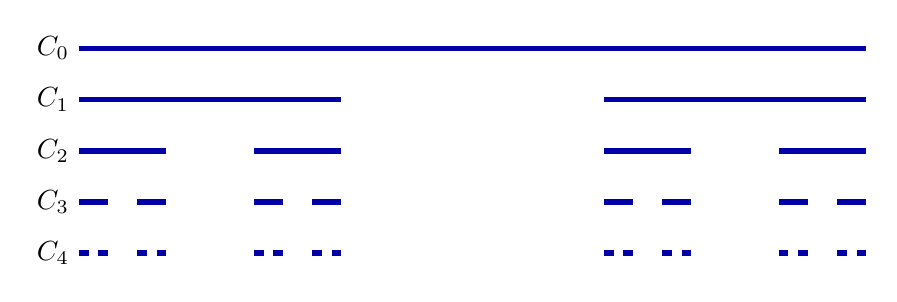
\begin{tikzpicture}[x=10cm,y=.65cm]
 \foreach \n in {0,...,4}{
  \node[left] at (0,-\n) {$C_{\n}$};
  \pgfmathtruncatemacro{\m}{2^\n-1}
  \foreach \j in {0,...,\m}{
   \pgfmathsetmacro{\a}{0}
   \ifnum\n>0
    \foreach \k in {1,...,\n}{
     \pgfmathtruncatemacro{\bit}{mod(floor(\j/2^(\n-\k)),2)}
     \pgfmathsetmacro{\temp}{\a+2*\bit/3^\k}
     \xdef\a{\temp}
    }
   \fi
   \draw[blue!65!black,line width=2pt] (\a,-\n)--({\a+3^(-\n)},-\n);
  }
 }
\end{tikzpicture}

\small Rysunek: pierwsze pięć etapów konstrukcji zbioru Cantora.
\end{center}

\section{Funkcja Cantora}
\begin{twierdzenie}
\label{ma1:thm:cantor-function}
Istnieje ciągła niemalejąca funkcja $F:[0,1]\to[0,1]$, dla której $F(0)=0$, $F(1)=1$ i która jest stała na każdym otwartym przedziale usuniętym w konstrukcji zbioru Cantora. Ponadto $F(C)=[0,1]$.
\end{twierdzenie}
\begin{proof}
Niech $F_0(x)=x$. Indukcyjnie załóżmy, że $F_n$ jest ciągła i niemalejąca, stała na wszystkich przedziałach usuniętych do etapu $n$, a na każdym przedziale składowym $[u,v]$ zbioru $C_n$ jest afiniczna i $F_n(v)-F_n(u)=2^{-n}$. Na $[u,v]$ definiujemy $F_{n+1}$ jako funkcję ciągłą, afiniczną na każdej z trzech równych części, o wartościach na kolejnych końcach tych części
\[
 F_n(u),\quad F_n(u)+2^{-(n+1)},\quad
 F_n(u)+2^{-(n+1)},\quad F_n(v).
\]
Poza $C_n$ pozostawiamy $F_{n+1}=F_n$. Na końcach przedziałów składowych nowe i stare wartości są zgodne. Wszystkie cztery wartości są uporządkowane niemalejąco; na każdej z pozostałych części wzrost jest równy $2^{-(n+1)}$. Skończenie wiele odcinków skleja się w ciągłą niemalejącą funkcję, co zamyka indukcję.

Różnica $F_{n+1}-F_n$ jest na każdej trzeciej części afiniczna. Na końcach przedziału $[u,v]$ jest równa zeru, a na dwóch punktach podziału odpowiednio $2^{-n}/6$ i $-2^{-n}/6$. Jej moduł na każdym z trzech odcinków nie przekracza największego modułu na końcach. Poza $C_n$ różnica jest zerowa. Zatem dla wszystkich $x\in[0,1]$,
\[
 |F_{n+1}(x)-F_n(x)|\le 2^{-n}/6.
\]
Dla $m>n$ nierówność trójkąta daje $|F_m(x)-F_n(x)|\le\sum_{k=n}^{m-1}2^{-k}/6\le 2^{-n}/3$. Dla każdego $x$ ciąg wartości jest ciągiem Cauchy'ego w $\R$, więc istnieje $F(x)=\lim_n F_n(x)$. Przechodząc w oszacowaniu do granicy $m\to\infty$, otrzymujemy $|F(x)-F_n(x)|\le2^{-n}/3$ dla wszystkich $x$.

Ustalmy $p\in[0,1]$ i $\varepsilon>0$. Wybierzmy $n$ z $2^{-n}/3<\varepsilon/3$. Z ciągłości $F_n$ istnieje $\delta>0$ takie, że $|F_n(x)-F_n(p)|<\varepsilon/3$ dla $|x-p|<\delta$ w dziedzinie. Wówczas
$|F(x)-F(p)|\le |F(x)-F_n(x)|+|F_n(x)-F_n(p)|+|F_n(p)-F(p)|<\varepsilon$.
To dowodzi ciągłości bez odwoływania się do późniejszej teorii zbieżności jednostajnej funkcji. Przejście do granicy zachowuje niemalejący charakter, wartości końcowe oraz stałość na każdym usuniętym przedziale, ponieważ od etapu jego usunięcia wszystkie późniejsze funkcje mają tam tę samą wartość.

Z twierdzenia o wartości pośredniej $F([0,1])=[0,1]$. Jeżeli $y=F(x)$ i $x\notin C$, to $x$ należy do pewnego usuniętego otwartego przedziału $(u,v)$. Jego końce należą do $C$, a ciągłość i stałość w $(u,v)$ dają $F(u)=F(x)=F(v)$. Zatem każda wartość z $[0,1]$ jest osiągana już na $C$.
\end{proof}
\begin{center}
\begin{tikzpicture}[x=8cm,y=4cm,>=Stealth]
 \draw[->] (-.03,0)--(1.08,0) node[right] {$x$};
 \draw[->] (0,-.05)--(0,1.1) node[above] {$y$};
 \draw[gray,dashed] (0,0)--(1,1);
 \draw[blue!65!black,thick] (0,0)--(1/27,1/8)--(2/27,1/8)--(1/9,1/4)--(2/9,1/4)--(7/27,3/8)--(8/27,3/8)--(1/3,1/2)--(2/3,1/2)--(19/27,5/8)--(20/27,5/8)--(7/9,3/4)--(8/9,3/4)--(25/27,7/8)--(26/27,7/8)--(1,1);
 \node[below] at (1,0) {$1$};
 \node[left] at (0,1) {$1$};
\end{tikzpicture}

\small Rysunek: trzecie przybliżenie $F_3$ funkcji Cantora; linia przerywana to $F_0$.
\end{center}
Funkcja Cantora nie jest stała, mimo że jest lokalnie stała na otwartym gęstym podzbiorze $[0,1]$ (dopełnieniu $C$ względem $[0,1]$). To odróżnia lokalną stałość na całej dziedzinie od lokalnej stałości tylko na zbiorze gęstym.

\section{Zbiory punktów ciągłości}
\begin{definicja}
\label{ma1:def:point-oscillation}
Niech $X,Y$ będą przestrzeniami metrycznymi, $f:X\to Y$ i $p\in X$. Oscylacją $f$ w $p$ nazywamy
\[
 \omega_f(p)=\inf_{r>0}\ \sup\{d_Y(f(x),f(y)):x,y\in B_X(p,r)\}.
\]
Kres górny dopuszcza wartość $+\infty$, a zbiór par jest zawsze niepusty.
\end{definicja}
\begin{twierdzenie}
\label{ma1:thm:continuity-gdelta}
Funkcja $f:X\to Y$ jest ciągła w $p$ wtedy i tylko wtedy, gdy $\omega_f(p)=0$. Dla każdego $\eta>0$ zbiór $U_\eta=\{p\in X:\omega_f(p)<\eta\}$ jest otwarty. W szczególności zbiór punktów ciągłości jest typu $G_\delta$ (przeliczalnym przecięciem zbiorów otwartych), a zbiór punktów nieciągłości jest typu $F_\sigma$ (przeliczalną sumą zbiorów domkniętych).
\end{twierdzenie}
\begin{proof}
Jeśli $f$ jest ciągła w $p$, to dla $\varepsilon>0$ wybieramy $r$ tak, aby $d_Y(f(x),f(p))<\varepsilon/3$ dla $x\in B_X(p,r)$. Z nierówności trójkąta średnica obrazu tej kuli jest nie większa niż $2\varepsilon/3<\varepsilon$. Stąd $\omega_f(p)=0$. Odwrotnie, jeśli $\omega_f(p)=0$, dla $\varepsilon>0$ wybieramy $r$ ze średnicą obrazu mniejszą niż $\varepsilon$. Ponieważ $p\in B_X(p,r)$, dla każdego $x$ z tej kuli mamy $d_Y(f(x),f(p))<\varepsilon$.

Jeżeli $p\in U_\eta$, istnieje $r>0$, dla którego średnica obrazu $B_X(p,r)$ jest mniejsza niż $\eta$. Dla $q\in B_X(p,r/2)$ nierówność trójkąta daje $B_X(q,r/2)\subseteq B_X(p,r)$. Średnica obrazu mniejszej kuli nie przekracza średnicy obrazu większej, więc $\omega_f(q)<\eta$. To dowodzi otwartości. Z pierwszej części i nieujemności oscylacji zbiór punktów ciągłości jest równy $\bigcap_{n\ge1}U_{1/n}$, a jego dopełnienie jest sumą zbiorów domkniętych $X\setminus U_{1/n}$.
\end{proof}

\begin{wniosek}
\label{ma1:cor:no-rational-continuity}
Nie istnieje funkcja $f:\R\to\R$ ciągła dokładnie w punktach wymiernych.
\end{wniosek}
\begin{proof}
Gdyby taka funkcja istniała, to $\Q=\bigcap_{n\ge1}U_n$ dla pewnych otwartych zbiorów $U_n\subseteq\R$. Każdy z nich zawiera $\Q$, więc jest gęsty. Niech $(r_n)_{n\ge1}$ będzie wyliczeniem liczb wymiernych. Zbiory $V_n=U_n\setminus\{r_n\}$ są otwarte i gęste: każde niepuste otwarte otoczenie przecina $U_n$ w niepustym otwartym zbiorze, który zawiera punkt różny od $r_n$.

Wybieramy indukcyjnie niepuste przedziały domknięte $I_n$ dodatniej długości: $I_0=[0,1]$, a $I_n$ zawiera się w $\operatorname{int} I_{n-1}\cap V_n$ i ma długość nie większą niż $1/n$. Wybór jest możliwy, gdyż przecięcie to jest niepustym zbiorem otwartym i zawiera pewien przedział o dodatniej długości. Twierdzenie o przedziałach zstępujących daje punkt $x$ należący do wszystkich $I_n$, a więc do wszystkich $V_n$. W konsekwencji $x\in\bigcap_n U_n=\Q$, ale $x\ne r_n$ dla każdego $n$. Sprzeczność.
\end{proof}
Jest to szczególny argument kategorii Baire'a w $\R$. Nie korzystamy z ogólnego twierdzenia Baire'a ani z teorii miary. Funkcja Thomae'a pokazuje, że odwrócona sytuacja, ciągłość dokładnie w punktach niewymiernych, jest możliwa.
